\documentclass[tikz,border=8pt]{standalone}
\usepackage{amsmath}
\usetikzlibrary{arrows.meta,decorations.pathreplacing}
\begin{document}

% Asset ID: AS2DataPresentationTikZ-005
% Source: Histogram gaps evidence.
% Related lesson section: Core Theory, Gaps and True Class Widths.
% Purpose: Convert written rounded classes into true intervals.
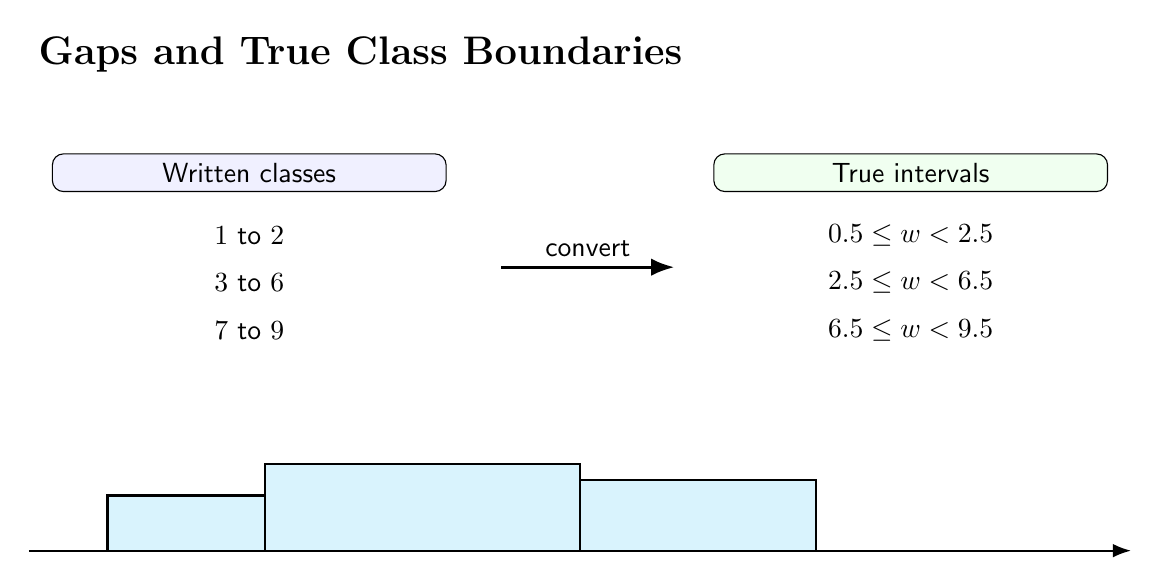
\begin{tikzpicture}[>=Latex,font=\sffamily]
\node[anchor=west,font=\bfseries\Large] at (0,7.3){Gaps and True Class Boundaries};
\node[draw,rounded corners,fill=blue!6,minimum width=5cm] at (2.8,5.8){Written classes};
\node at (2.8,5.0){$1$ to $2$}; \node at (2.8,4.4){$3$ to $6$}; \node at (2.8,3.8){$7$ to $9$};
\draw[->,very thick] (6,4.6)--(8.2,4.6) node[midway,above]{convert};
\node[draw,rounded corners,fill=green!6,minimum width=5cm] at (11.2,5.8){True intervals};
\node at (11.2,5.0){$0.5\leq w<2.5$}; \node at (11.2,4.4){$2.5\leq w<6.5$}; \node at (11.2,3.8){$6.5\leq w<9.5$};
\draw[->,thick] (0,1)--(14,1); \draw[fill=cyan!15,thick] (1,1) rectangle (3,1.7); \draw[fill=cyan!15,thick] (3,1) rectangle (7,2.1); \draw[fill=cyan!15,thick] (7,1) rectangle (10,1.9);
\end{tikzpicture}

\end{document}
